Après optimisation, on obtient que le modèle ayant le mieux performer en validation est un celui avec un objet de compte binaire (0 ou 1) qui utilise des 1 gramme et qui conserve une fréquence minimale de 2 mots. Le modèle de classification utilisé est une régression logistique avec une pénalité de choix de paramètres \emph{L1}:

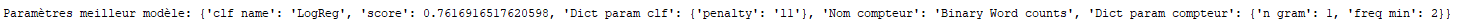
\includegraphics[width=\linewidth,height=1cm,keepaspectratio]{images/dict_meilleur_model}

On peut évaluer notre modèle en calculant le score qu'on obtiendrait sur 80\% de notre corpus d'entraînement qui sert d'entraînement, et 20 \% qui sert de test. Avec notre meilleur modèle, on obtient les résultats suivants:

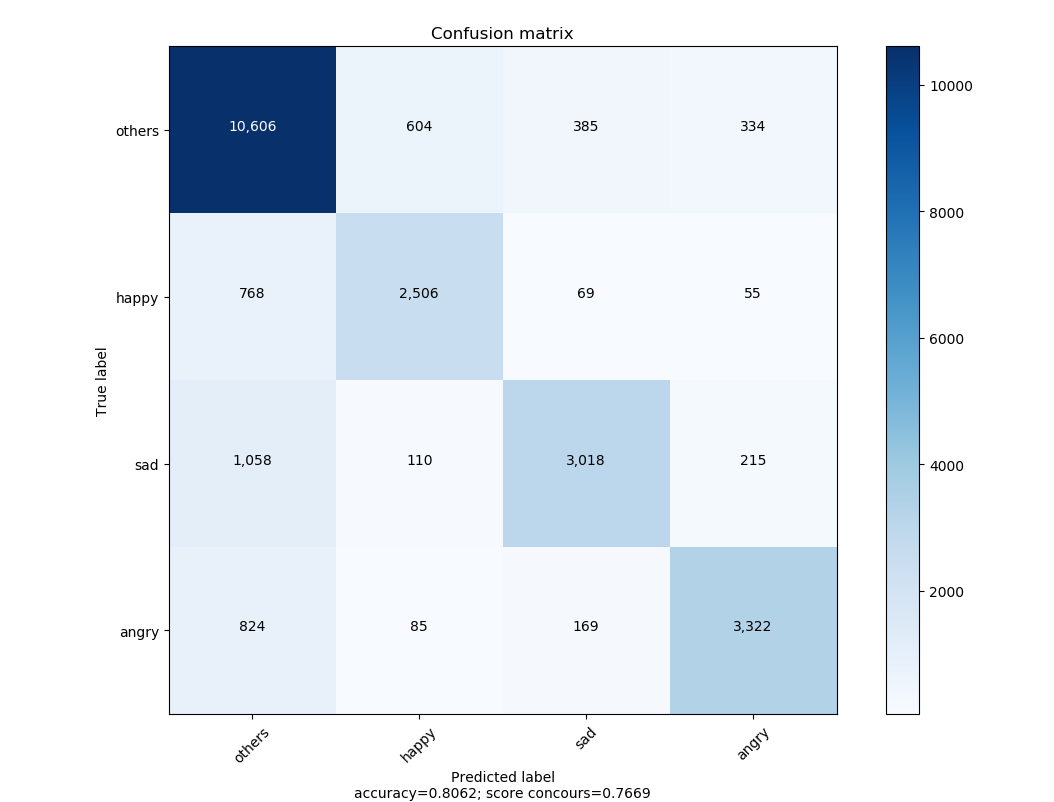
\includegraphics[width=\linewidth,keepaspectratio]{images/confusion_matrix_avec_features}

On peut voir que le score utilisé par le concours de 0.7669 est quand même assez haut. On remarque que la plupart des erreurs faites sont majoritairement de prédire happy, sad et angry comme étant others. De plus, la confusion entre sad et angy est un peu plus élevée qu'entre les autres paires d'émotions puisque qu'on peut supposer que les deux sont à caractère négatif.

On peut également observer la matrice de confusion lorsque l'on n'ajoute pas les variables d'emoji et de binettes:

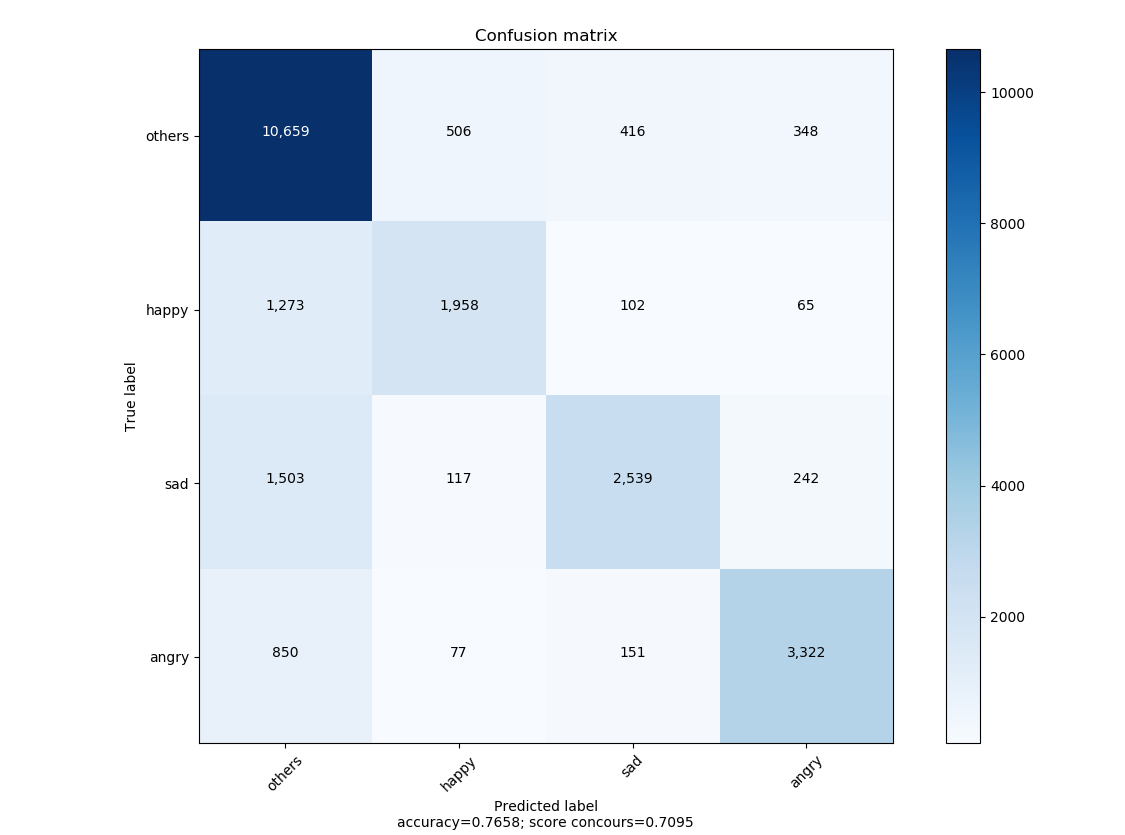
\includegraphics[width=\linewidth,keepaspectratio]{images/confusion_matrix_sans_features}
On voit tout de suite que le score est beaucoup moins bon (0.7095 au lieu de 0.7669). On peut voir que beaucoup plus de classe happy et sad ont été prédites comme étant others (768 à 1273 et 1058 à 1503). Pour ce qui est de angry, les nombres changent très peu, on peut  supposer qu'il y a très peu d'emojis et de binettes dans notre corpus de test pour la classe angry.

Encore une fois, on peut supposer que notre modèle avec les variables ajoutées est meilleur que celui sans, à cause du meilleur score. On peut également comparer notre score aux meilleurs scores soumis à la compétition:

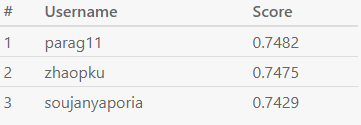
\includegraphics[width=\linewidth,height=4cm,keepaspectratio]{images/meilleurs_scores}

On peut conclure qu'un score de 0.7669 en simulation de test est donc très bon. Il est toutefois difficile de bien comparer puisque la répartition des classes n'est pas la même dans le corpus à prédire. Le fichier de test avait environ 16.6\% de happy, sad, angry et 50\% de others, alors que le fichier à prédire a des proportions de 4\% et 88\%. 

On peut quand même être réellement satisfait du résultat puisque cela ne devrait pas trop affecter nos prédictions.